
\documentclass[14pt, a4paper]{article}
\usepackage{minitoc}
\usepackage[left=3.00cm, right=2.5cm, top=2.00cm, bottom=2.00cm]{geometry}
\usepackage{amsmath}
\usepackage{amssymb}
\usepackage{amsthm}
\usepackage{thmtools}
\usepackage{mathtools}
\usepackage{graphicx}
%\usepackage{algpseudocode}
%\usepackage{algorithm}
\usepackage[ruled,vlined,linesnumbered,algosection]{algorithm2e}
\usepackage{blindtext}
\usepackage{setspace}
\usepackage[utf8]{inputenc}
\usepackage[utf8]{vietnam}
\usepackage[center]{caption}
\usepackage[shortlabels]{enumitem}
\usepackage{fancyhdr} % header, footer
\usepackage{hyperref} % loại bỏ border với mục lục và công thức
\usepackage[nonumberlist, nopostdot, nogroupskip]{glossaries}
\usepackage{glossary-superragged}
\usepackage{tikz,tkz-tab}
\setglossarystyle{superraggedheaderborder}
\pagestyle{fancy}
%\usepackage[style=numeric,sortcites]{biblatex}
%\addbibresource{ref.bib}
%\usepackage[numbers]{natbib}
\usepackage{indentfirst}
\usepackage{multirow}
\usepackage[natbib,backend=biber,style=ieee, sorting=ynt]{biblatex}
\bibliography{ref.bib}

\usepackage{caption}
\usepackage{subcaption}

\graphicspath{{./figures/}}


\makenoidxglossaries

% Danh mục thuật ngữ

\hypersetup{
    colorlinks=false,
    pdfborder={0 0 0},
}


\fancyhf{}
\rhead{\textbf{Môn học: Một số vấn đề về đồ họa máy tính}}
\lhead{\textbf{GVHD: TS. Nguyễn Thị Bích Thủy}}
\rfoot{\thepage}
\lfoot{\textbf{Học viên thực hiện: Nguyễn Chí Thanh - 21007925}}
\renewcommand{\headrulewidth}{0.4pt}
\renewcommand{\footrulewidth}{0.4pt}


\numberwithin{equation}{section}
\numberwithin{figure}{section}

\setlength{\parindent}{0.5cm}

\setcounter{secnumdepth}{3} % Cho phép subsubsection trong report
\setcounter{tocdepth}{3} % Chèn subsubsection vào bảng mục lục

\newtheorem{dl}{Định lý}
\newtheorem{md}{Mệnh đề}
\newtheorem{bd}{Bổ đề}
\newtheorem{dn}{Định nghĩa}
\newtheorem{hq}{Hệ quả}

\numberwithin{dl}{section}
\numberwithin{md}{section}
\numberwithin{bd}{section}
\numberwithin{dn}{section}
\numberwithin{hq}{section}

\doublespacing
\AtBeginEnvironment{tabular}{\doublespacing}


\begin{document}
    \begin{titlepage}

        \newcommand{\HRule}{\rule{\linewidth}{0.5mm}} % Defines a new command for the horizontal lines, change thickness here

        \center % Center everything on the page

        %----------------------------------------------------------------------------------------
        %	HEADING SECTIONS
        %----------------------------------------------------------------------------------------
        \textsc{\LARGE Đại học Quốc Gia Hà Nội}\\[0.5cm]
        \textsc{\LARGE Trường đại học Khoa học tự nhiên}\\[0.5cm] % Name of your university/college
        \textsc{\LARGE Khoa Toán - Cơ - Tin học}\\[0.5cm]

        
\includegraphics[scale=0.2]{HUS-logo.jpg}\\[0.5cm]

        \textsc{\Large Chuyên ngành: Khoa học dữ liệu}\\[0.5cm] % Major heading such as course name


        %----------------------------------------------------------------------------------------
        %	TITLE SECTION
        %----------------------------------------------------------------------------------------

        \HRule \\[0.4cm]
        { \huge \bfseries BÀI TẬP MÔN HỌC}\\[0.4cm] % Title of your document
        \HRule \\[1.5cm]

        \textsc{\Large Môn học: Một số vấn đề về đồ họa máy tính}\\[1cm] % Minor heading such as course title


        \textsc{\Large Đề tài: Phân tích dữ liệu cuộc bầu cử \\ Tổng thống Mỹ năm 2020}\\[2cm]


        %----------------------------------------------------------------------------------------
        %	AUTHOR SECTION
        %----------------------------------------------------------------------------------------
        \begin{minipage}{0.4\textwidth}
            \begin{flushleft} \large
            \emph{Giảng viên hướng dẫn:} \\
            TS. Nguyễn Thị Bích Thủy % Supervisor's Name
            \end{flushleft}
        \end{minipage}\\[0.5cm]

        \begin{minipage}{0.4\textwidth}
        \begin{flushleft} \large
        \emph{Học viên thực hiện:}\\
        Nguyễn Chí Thanh \\
        MSHV: 21007925 \\ % Your name
        Lớp: Khoa học dữ liệu - K4
        \end{flushleft}
        \end{minipage}


        % If you don't want a supervisor, uncomment the two lines below and remove the section above
        %\Large \emph{Author:}\\
        %John \textsc{Smith}\\[3cm] % Your name

        %----------------------------------------------------------------------------------------
        %	DATE SECTION
        %----------------------------------------------------------------------------------------

        % I don't want day because it is English
        % {\large \today}\\[2cm] % Date, change the \today to a set date if you want to be precise

        %----------------------------------------------------------------------------------------
        %	LOGO SECTION
        %----------------------------------------------------------------------------------------

        %\includegraphics{logo/rsz_3logo-khtn.png}\\[1cm] % Include a department/university logo - this will require the graphicx package

        %----------------------------------------------------------------------------------------

        \vfill % Fill the rest of the page with whitespace

    \end{titlepage}

    \cleardoublepage
    \pagenumbering{gobble}
    \tableofcontents
    \newpage
    \listoffigures
    \newpage
    \glsaddall 
    \renewcommand*{\glossaryname}{Danh mục các từ viết tắt}
    \renewcommand*{\acronymname}{Danh sách từ viết tắt}
    \renewcommand*{\entryname}{Viết tắt}
    \renewcommand*{\descriptionname}{Viết đầy đủ}
    \printnoidxglossary
    \cleardoublepage
    \pagenumbering{arabic}

    %\maketitle

    \newpage

    \nocite{*}

    \begin{center}
    \section*{LỜI MỞ ĐẦU}
    \end{center}
    \addcontentsline{toc}{section}{{\bf LỜI MỞ ĐẦU}\rm}


    \newpage

    \section{Tổng quan về cuộc bầu cử tổng thống Mỹ năm 2020}

    \subsection{Diễn biến chính của cuộc bầu cử}

    Cuộc bầu cử tổng thống Hoa Kỳ năm 2020 là cuộc bầu cử tổng thống lần thứ 59, được tổ chức vào Thứ Ba, ngày 3 tháng 11 năm 2020. Lá phiếu của đảng Dân chủ thuộc về cựu phó tổng thống Joe Biden và hạ nghị sĩ Hoa Kỳ đến từ California Kamala Harris đã đánh bại tổng thống đương nhiệm của đảng Cộng hòa Donald Trump và phó tổng thống đương nhiệm Mike Pence. 
    Cuộc bầu cử diễn ra trong bối cảnh đại dịch COVID-19 toàn cầu và suy thoái kinh tế. 
    Đây là cuộc bầu cử đầu tiên kể từ năm 1992 mà tổng thống đương nhiệm không giành được nhiệm kỳ thứ hai. 
    Cuộc bầu cử chứng kiến tỷ lệ cử tri đi bầu cao nhất tính theo tỷ lệ phần trăm kể từ năm 1900, với mỗi ứng cử viên trong số hai ứng cử viên chính nhận được hơn 74 triệu phiếu bầu, vượt qua kỷ lục 69,5 triệu phiếu bầu của Barack Obama từ năm 2008. 
    Biden nhận được hơn 81 triệu phiếu bầu, số phiếu bầu nhiều nhất từng bầu cho một ứng cử viên trong cuộc bầu cử tổng thống Hoa Kỳ.

    Trong một cuộc bầu cử sơ bộ mang tính cạnh tranh có nhiều ứng cử viên nhất cho bất kỳ đảng chính trị nào trong kỷ nguyên hiện đại của nền chính trị Hoa Kỳ, Joe Biden đã giành được đề cử tổng thống của đảng Dân chủ trước đối thủ gần nhất của mình, Thượng nghị sĩ Bernie Sanders. 
    Người bạn tranh cử của Joe Biden, Kamala Harris, đã trở thành ứng cử viên phó tổng thống người Mỹ gốc Phi đầu tiên, người Mỹ gốc Á đầu tiên và là phụ nữ thứ ba giành chiến thắng trong một đảng lớn. 
    Trump giành được sự tái đề cử, nhận được tổng cộng 2.549 đại biểu, một trong những con số nhiều nhất trong lịch sử cuộc chạy đua sơ bộ tranh cử tổng thống, so với người về nhì là Bill Weld, một đại biểu trong các cuộc bầu cử sơ bộ của Đảng Cộng hòa. 
    Jo Jorgensen đã giành được đề cử tổng thống Đảng Tự do với Spike Cohen là người bạn tranh cử của Jorgensen và Howie Hawkins đã giành được đề cử tổng thống Đảng Xanh với Angela Nicole Walker là người bạn tranh cử của Hawkins.

    Các vấn đề trọng tâm của cuộc bầu cử bao gồm các tác động kinh tế và sức khỏe cộng đồng khi đại dịch COVID-19 đang diễn ra, tình trạng bất ổn trước vụ cảnh sát sát hại George Floyd.
    Tương lai của Đạo luật điều chỉnh giá cả hợp lý. Do đại dịch đang diễn ra, số lượng phiếu bầu đã được bỏ sớm và qua đường bưu điện ở mức kỷ lục. 
    Nhiều đảng viên Đảng Dân chủ đã đăng ký bỏ phiếu qua thư hơn những đảng viên Đảng Cộng hòa. 
    Do có một số lượng lớn các lá phiếu gửi qua thư, một số bang đã gặp phải sự chậm trễ trong việc kiểm phiếu và báo cáo,
    điều này dẫn đến việc các hãng tin lớn trì hoãn dự đoán Biden và Harris là tổng thống đắc cử và phó tổng thống đắc cử cho đến sáng ngày 7 tháng 11, ba ngày sau cuộc bầu cử. 
    Các hãng truyền thông lớn dự đoán một ứng cử viên giành chiến thắng trên một tiểu bang khi một tỷ lệ lớn của phiếu đã được kiểm và ứng cử viên đó đang có tỷ lệ phiếu áp đảo so với các ứng cử viên còn lại.

    Cuối cùng, ông Biden đã giành được đa số trong Đại cử tri đoàn với 306 phiếu đại cử tri, trong khi ông Trump nhận được 232. 
    Quyết định dẫn đến chiến thắng của Biden là chiến thắng của ông ở các bang Great Lakes nghiêng về đảng Dân chủ là Michigan, Pennsylvania và Wisconsin, những bang mà Trump đã giành được vào năm 2016 và cộng lại 46 phiếu đại cử tri là đủ để xoay chuyển cuộc bầu cử cho một trong hai ứng cử viên. 
    Biden cũng trở thành đảng viên Đảng Dân chủ đầu tiên giành chiến thắng trong cuộc bầu cử tổng thống ở Georgia kể từ năm 1992, ở Arizona từ năm 1996 và ở khu vực bầu cử số 2 của Nebraska kể từ năm 2008.

    Trước, trong và sau Ngày bầu cử, Trump và nhiều đảng viên Cộng hòa khác đã cố gắng lật tẩy cuộc bầu cử và lật ngược kết quả, cáo buộc sai sự thật về hành vi gian lận cử tri phổ thông và cố gắng tác động đến quá trình kiểm phiếu ở các bang. 
    Tổng đốc William Barr và các quan chức ở mỗi bang trong số 50 bang không tìm thấy bằng chứng nào về gian lận phiếu phổ phổ thông hoặc những bất thường trong cuộc bầu cử. 
    Các cơ quan liên bang giám sát an ninh bầu cử cho biết đây là cuộc bầu cử an toàn nhất trong lịch sử nước Mỹ. 
    Chiến dịch tranh cử của Trump và các đảng viên đảng Cộng hòa, bao gồm cả các thành viên Quốc hội của Đảng Cộng hòa, tiếp tục tham gia vào nhiều nỗ lực nhằm lật ngược kết quả bầu cử bằng cách đệ trình 63 vụ kiện ở một số bang (nhưng tất cả đều bị rút lại hoặc bác bỏ), 
    Các đảng viên đảng Cộng hòa cố gắng tuyên truyền các thuyết âm mưu cáo buộc gian lận để gây sức ép với các quan chức bầu cử cấp bang của Đảng Cộng hòa (đáng chú ý là Ngoại trưởng Georgia Brad Raffensperger, trong một cuộc điện thoại mà sau này được công bố rộng rãi) và các nhà lập pháp để thay đổi kết quả.
    Ngoài ra các đảng viên đảng Cộng hòa gây áp lực buộc Bộ Tư pháp tuyên bố cuộc bầu cử là "có gian lận" và cần phải được can thiệp, phản đối chứng nhận Đại Cử tri đoàn tại Quốc hội và từ chối hợp tác với quá trình chuyển giao tổng thống của Joe Biden. 
    Vụ viện lên đến đỉnh điểm khi một đám đông những người ủng hộ Trump tấn công Điện Capitol của Hoa Kỳ vào ngày 6 tháng 1 năm 2021, sau khi ông Trump liên tục nói rằng ông sẽ không bao giờ thừa nhận kết quả cuộc bầu cử. 
    Vào ngày 7 tháng 1, ông Trump thừa nhận chính quyền sắp tới mà không nhắc đến tên của Biden.
    Ông Biden và Harris được nhậm chức vào ngày 20 tháng 1 năm 2021.

    \subsection{Các ứng cử viên tranh cử tổng thống của từng Đảng}

    \subsection{Đảng Dân chủ}

    Joe Biden trở thành ứng cử viên giả định của Đảng Dân chủ vào ngày 5 tháng 6 năm 2020, khi ông có đủ số đại biểu để đảm bảo được đề cử tại đại hội toàn quốc. 
    Ông chính thức được đề cử tại hội nghị vào ngày 18 tháng 8 cùng năm.

    \begin{figure}[h!]
        \centering
        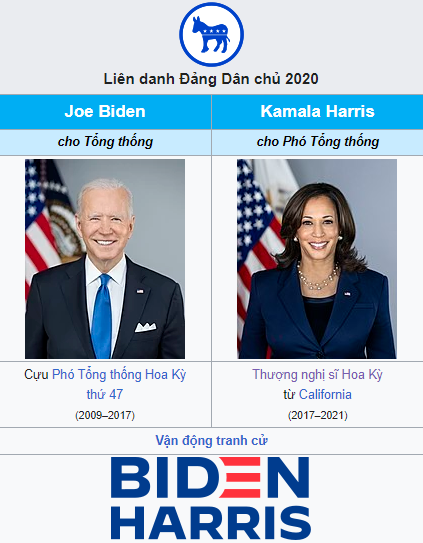
\includegraphics[width=0.6\textwidth]{Dem_Candidates.png}
        \caption{Ứng cử viên Tổng thống và ứng cử viên Phó Tổng thống Đảng Dân chủ}
    \end{figure}

    \subsection{Đảng Cộng hòa}

    Donald Trump và người bạn tranh cử Phó Tổng thống của ông, Mike Pence, đã có thể dễ dàng giành được đề cử sau khi nhận đủ số phiếu đại biểu trong cuộc bầu cử sơ bộ tổng thống của Đảng Cộng hòa năm 2020.

    \begin{figure}[h!]
        \centering
        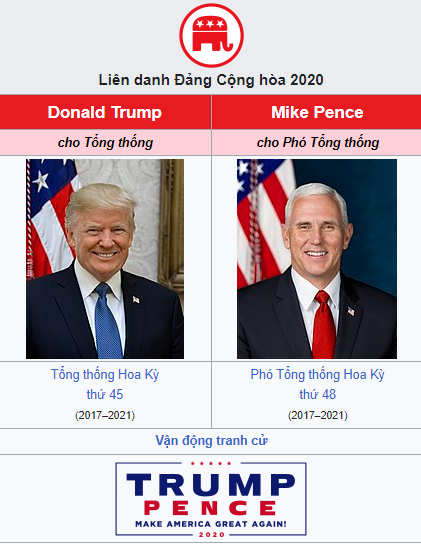
\includegraphics[width=0.6\textwidth]{Rep_Candidates.png}
        \caption{Ứng cử viên Tổng thống và ứng cử viên Phó Tổng thống Đảng Cộng hòa}
    \end{figure}

    \subsection{Đảng Tự do}

    Jo Jorgensen, người cùng tranh cử với Harry Browne vào năm 1996, đã nhận được đề cử của Đảng Tự do tại đại hội toàn quốc vào ngày 23 tháng 5 năm 2020.
    Bà đã đạt được quyền tiếp cận lá phiếu ở tất cả 50 tiểu bang và Quận Columbia.

    \begin{figure}[h!]
        \centering
        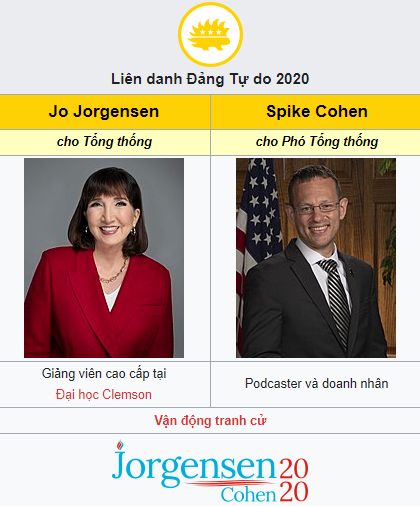
\includegraphics[width=0.6\textwidth]{Lib_Candidates.png}
        \caption{Ứng cử viên Tổng thống và ứng cử viên Phó Tổng thống Đảng Tự do}
    \end{figure}

    \subsection{Đảng Xanh}

    Howie Hawkins trở thành ứng cử viên giả định của Đảng Xanh vào ngày 21 tháng 6 năm 2020 và được đảng chính thức đề cử vào ngày 11 tháng 7 năm 2020.

    \begin{figure}[h!]
        \centering
        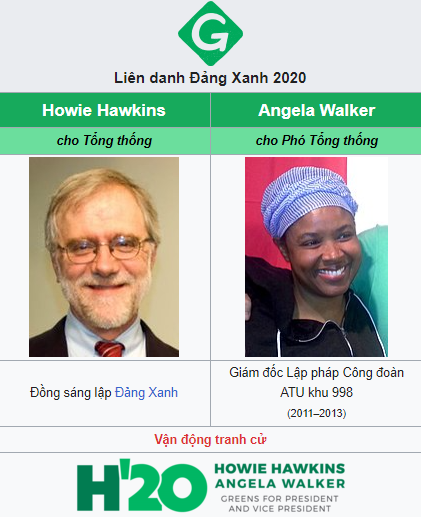
\includegraphics[width=0.6\textwidth]{Green_Candidates.png}
        \caption{Ứng cử viên Tổng thống và ứng cử viên Phó Tổng thống Đảng Xanh}
    \end{figure}

    \section{Trực quan hóa dữ liệu kết quả cuộc bầu cử Tổng thống năm 2020}


    \begin{figure}[h!]
        \centering
        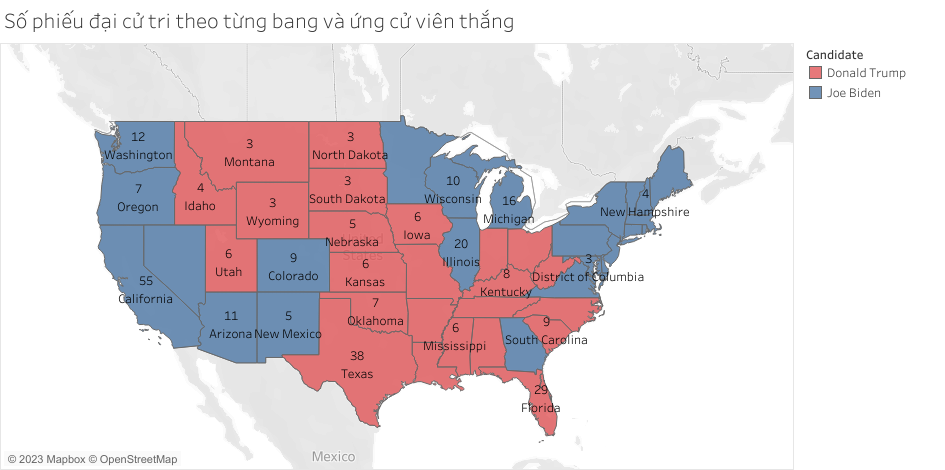
\includegraphics[width=0.9\textwidth]{Electoral_Votes_States.png}
        \caption{Số phiếu đại cử tri theo từng bang và ứng cử viên thắng}
    \end{figure}

    \begin{figure}[h!]
        \centering
        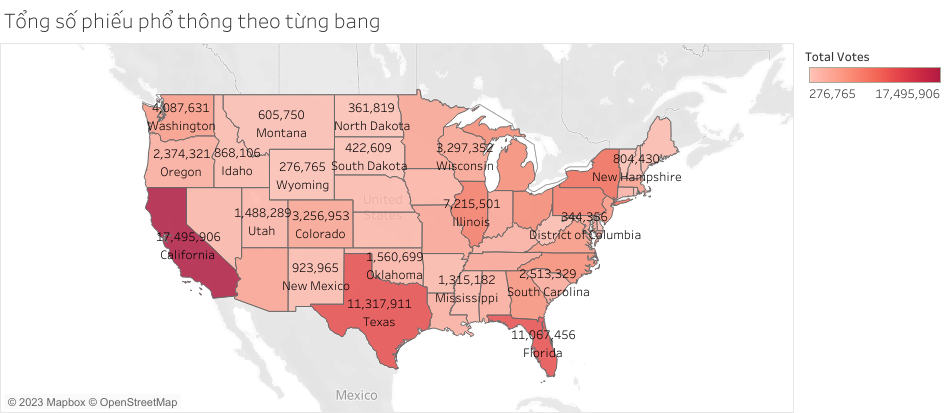
\includegraphics[width=0.9\textwidth]{Popular_Votes_States_by_Color.png}
        \caption{Tổng số phiếu phổ thông theo từng bang}
    \end{figure}

    \begin{figure}[h!]
        \centering
        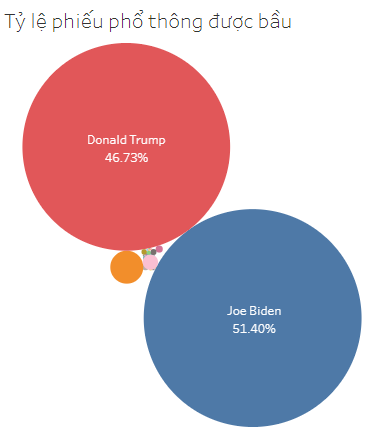
\includegraphics[width=0.6\textwidth]{Percentage_Total_Candidates_Bubble_Chart.png}
        \caption{Tỷ lệ phiếu phổ thông được bầu của từng ứng cử viên}
    \end{figure}

    \begin{figure}[h!]
        \centering
        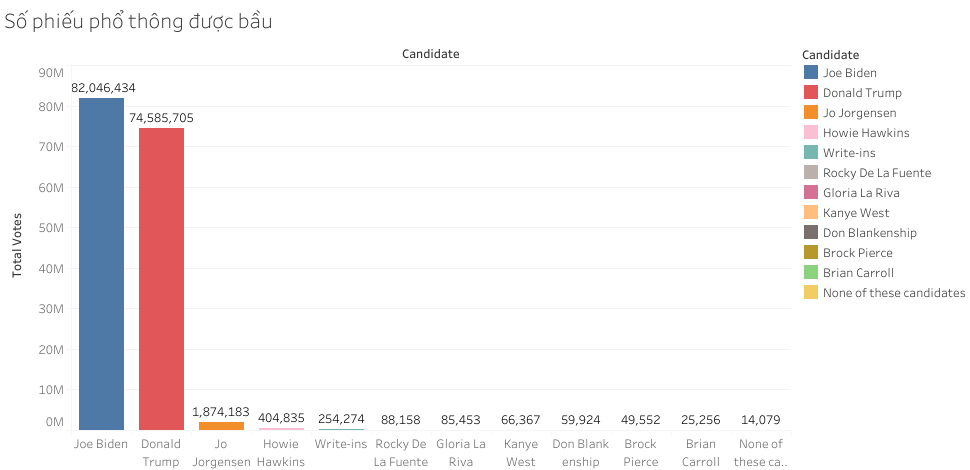
\includegraphics[width=0.9\textwidth]{Total_Popular_Votes_Candidates_Bar_Chart.png}
        \caption{Tổng số phiếu phổ thông được bầu của từng ứng cử viên}
    \end{figure}

    \begin{figure}[h!]
        \centering
        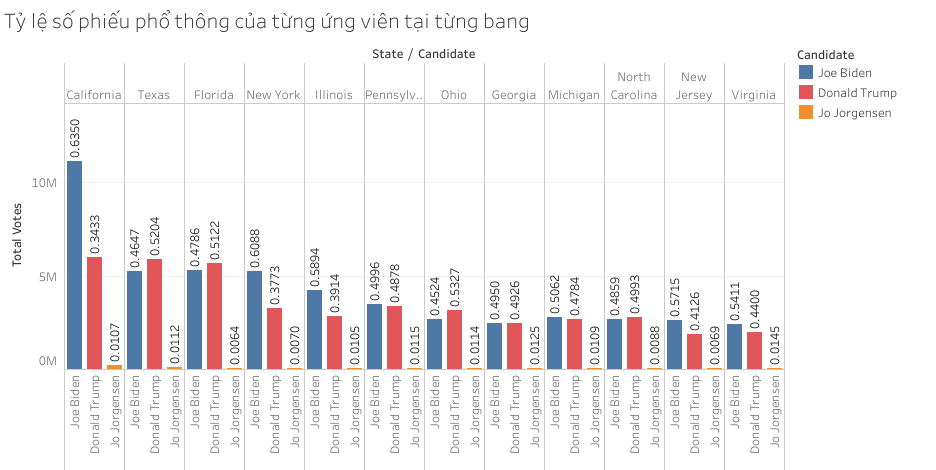
\includegraphics[width=0.9\textwidth]{Percentage_Popular_Votes_Candidates_by_States.png}
        \caption{Tỷ lệ số phiếu phổ thông của từng ứng viên tại từng bang}
    \end{figure}

    \begin{figure}[h!]
        \centering
        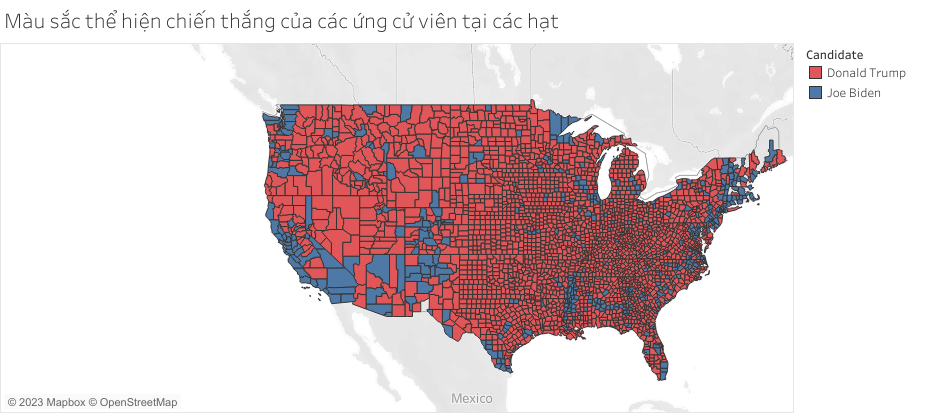
\includegraphics[width=0.9\textwidth]{County_Candidate_Win.png}
        \caption{Màu sắc thể hiện chiến thắng của các ứng cử viên tại các hạt}
    \end{figure}

    \begin{figure}[h!]
        \centering
        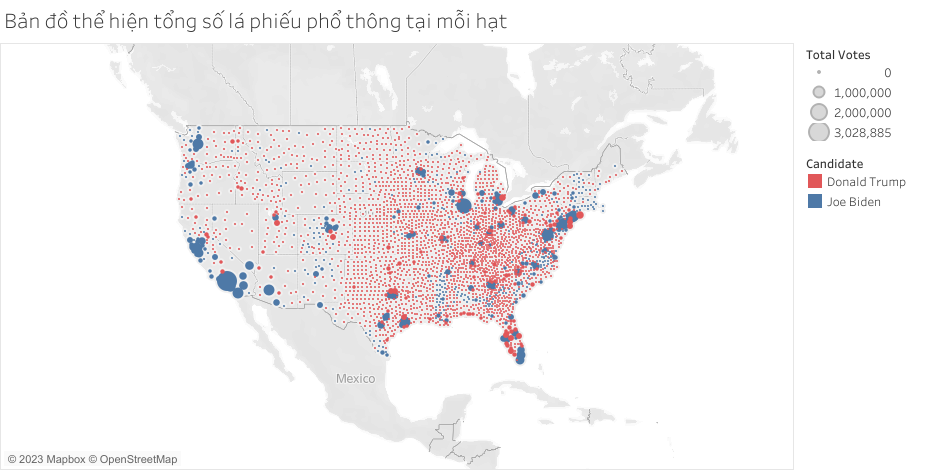
\includegraphics[width=0.9\textwidth]{County_Total_Vote_Circle.png}
        \caption{Bản đồ thể hiện tổng số lá phiếu phổ thông tại mỗi hạt}
    \end{figure}

    \begin{figure}[h!]
        \centering
        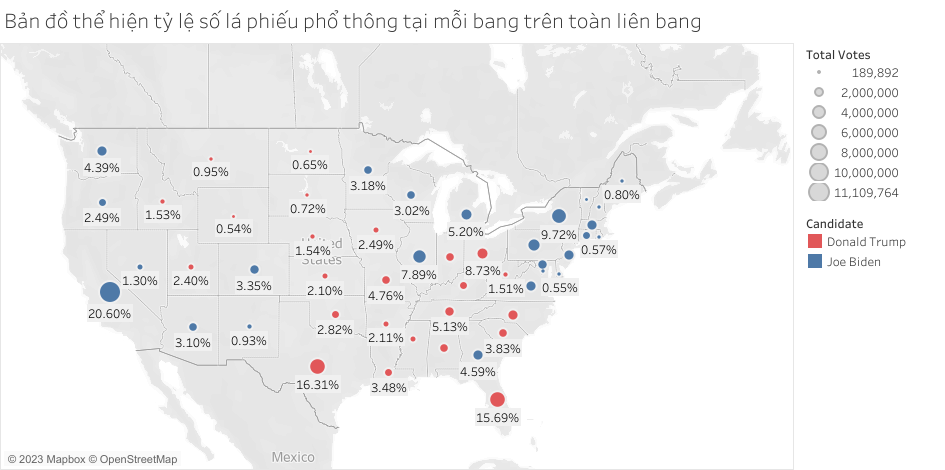
\includegraphics[width=0.9\textwidth]{State_Percentage_Vote_Circle.png}
        \caption{Bản đồ thể hiện tỷ lệ số lá phiếu phổ thông tại mỗi bang trên toàn liên bang}
    \end{figure}

    \begin{figure}[h!]
        \centering
        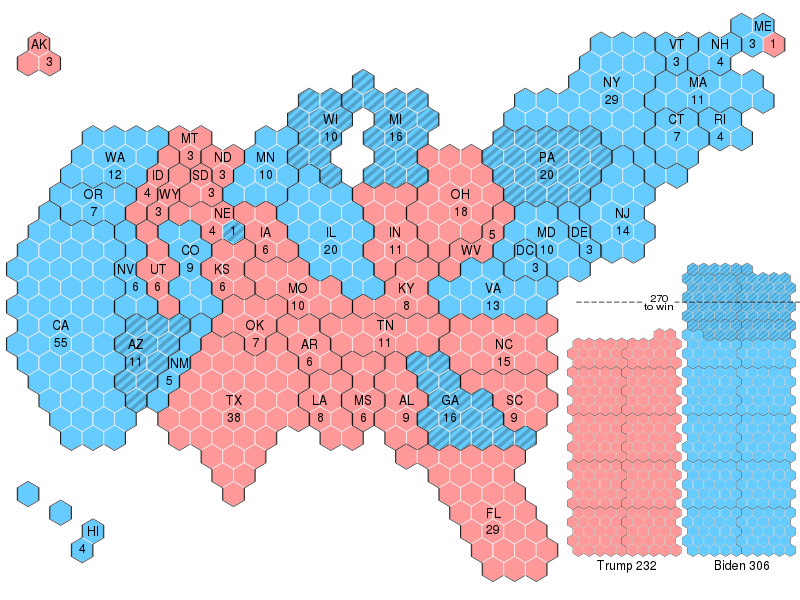
\includegraphics[width=0.9\textwidth]{State_Total_Vote_Cartogram.png}
        \caption{Cartogram thể hiện tổng số lá phiếu phổ thông tương ứng với các ứng cử viên thắng cuộc}
    \end{figure}

    \begin{figure}[h!]
        \centering
        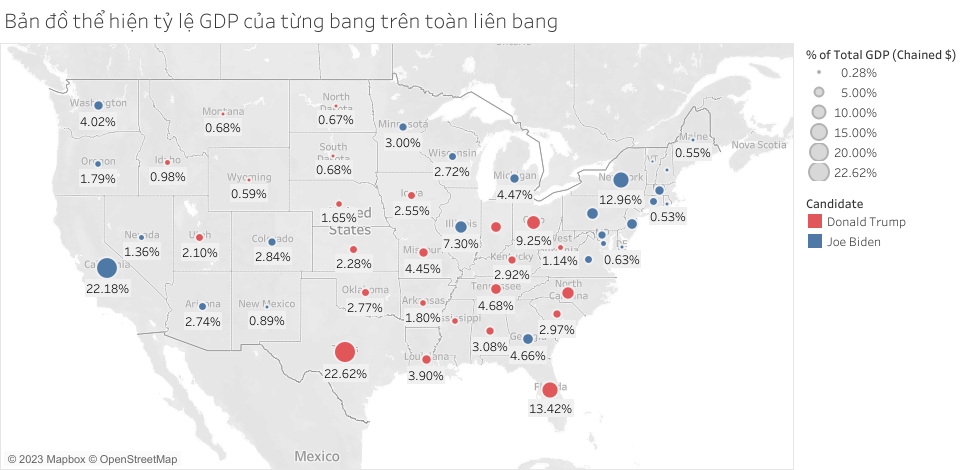
\includegraphics[width=0.9\textwidth]{figures/State_Percentage_GDP_Circle.png}
        \caption{Tỷ lệ GDP của tiểu bang trên toàn liên bang}
    \end{figure}

    \begin{figure}[h!]
        \centering
        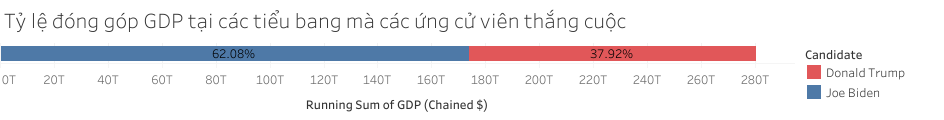
\includegraphics[width=0.9\textwidth]{State_Percentage_GDP_Candidate.png}
        \caption{Tỷ lệ đóng góp GDP tại các tiểu bang mà các ứng cử viên thắng}
    \end{figure}

    \begin{figure}[h!]
        \centering
        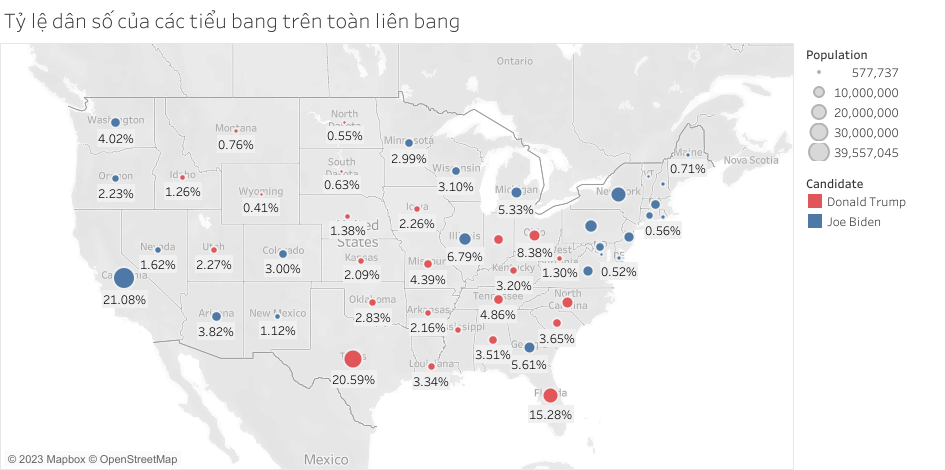
\includegraphics[width=0.9\textwidth]{State_Percentage_Population_Circle.png}
        \caption{Tỷ lệ dân số của tiểu bang trên toàn liên bang}
    \end{figure}

    \begin{figure}[h!]
        \centering
        \includegraphics[width=0.9\textwidth]{figures/State_Percentage_Population_Candidate.png}
        \caption{Tỷ lệ đóng góp dân số tại các tiểu bang mà các ứng cử viên thắng}
    \end{figure}

    \begin{figure}[h!]
        \centering
        \includegraphics[width=0.9\textwidth]{figures/County_Total_Percentage_Candidate_Win.png}
        \caption{Tỷ lệ thắng trên các hạt của từng ứng cử viên}
    \end{figure}

    \begin{figure}[h!]
        \centering
        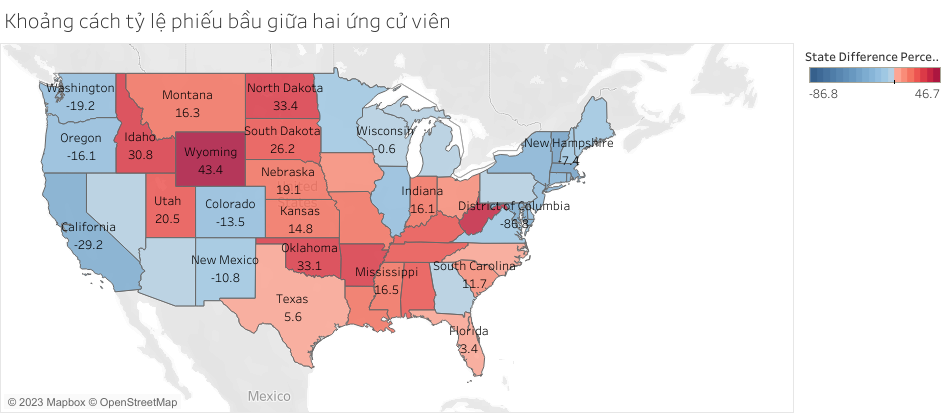
\includegraphics[width=0.9\textwidth]{figures/State_Difference_Percentage_Total_Vote_Two_Candidate.png}
        \caption{Khoảng cách tỷ lệ phiếu bầu giữa hai ứng cử viên tại các bang}
    \end{figure}

    \begin{figure}[h!]
        \centering
        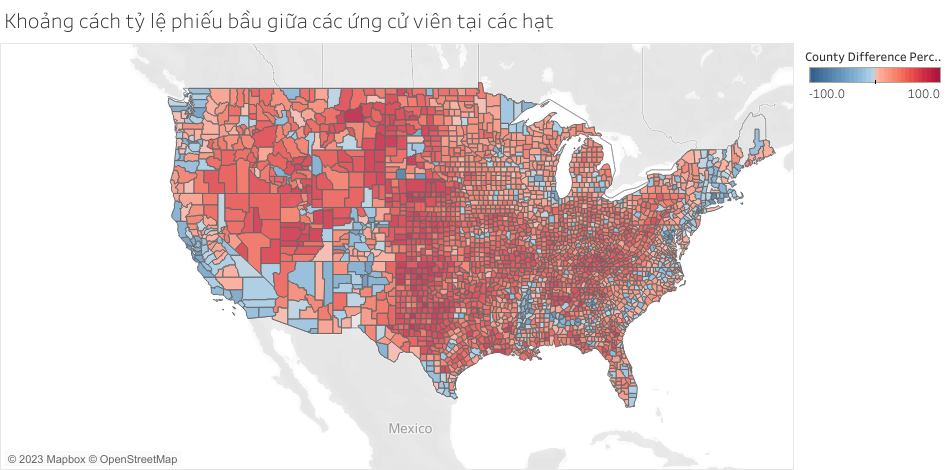
\includegraphics[width=0.9\textwidth]{figures/County_Difference_Percentage_Total_Vote_Two_Candidate.png}
        \caption{Khoảng cách tỷ lệ phiếu bầu giữa các ứng cử viên tại các hạt}
    \end{figure}

    \begin{figure}[h!]
        \centering
        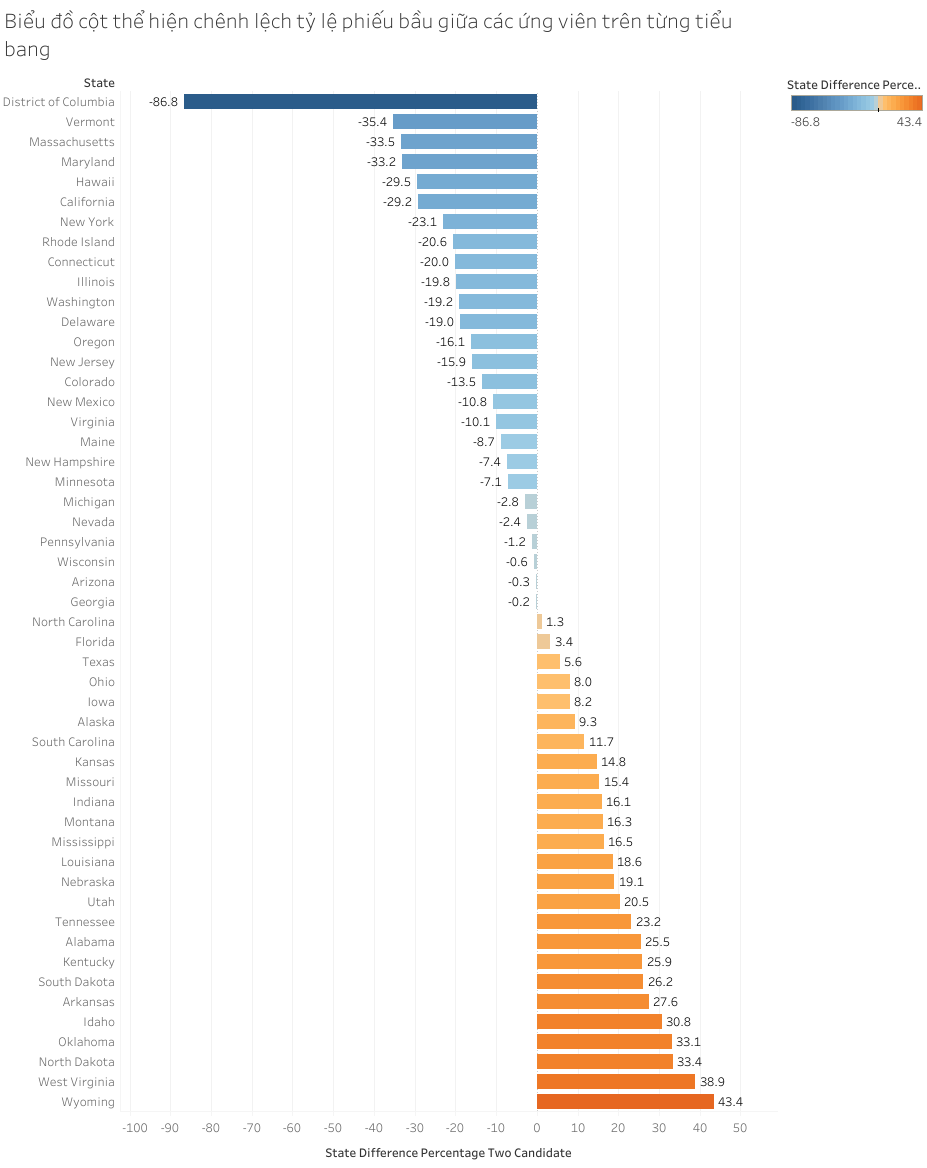
\includegraphics[width=0.9\textwidth]{figures/State_Difference_Percentage_Total_Vote_Two_Candidate_Bar_Chart.png}
        \caption{Biểu đồ cột thể hiện chênh lệch tỷ lệ phiếu bầu giữa các ứng viên trên từng tiểu bang}
    \end{figure}

    \begin{figure}[h!]
        \centering
        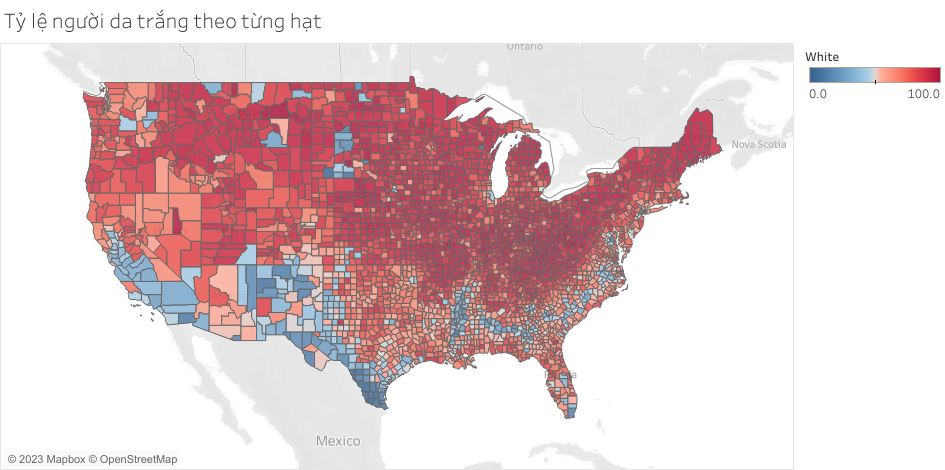
\includegraphics[width=0.9\textwidth]{figures/County_Percentage_White_People.png}
        \caption{Tỷ lệ người da trắng theo từng hạt}
    \end{figure}

    \begin{figure}[h!]
        \centering
        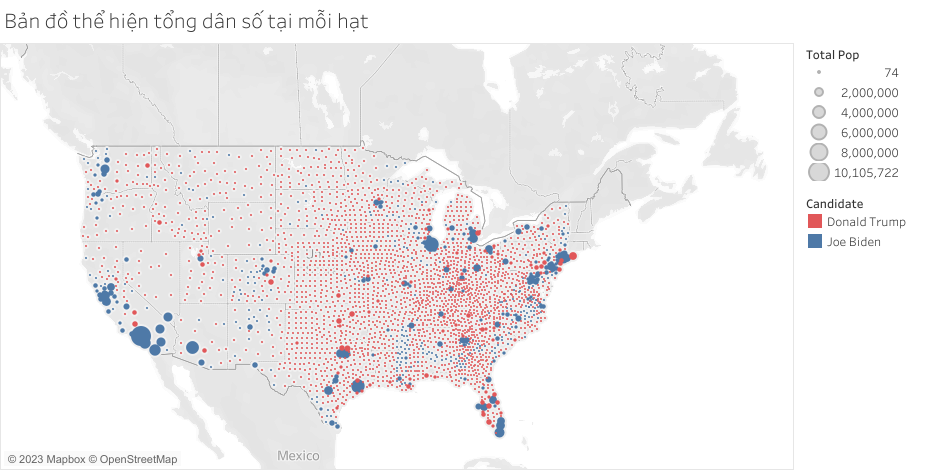
\includegraphics[width=0.9\textwidth]{figures/County_Total_Population_Circle.png}
        \caption{Bản đồ thể hiện tổng dân số tại mỗi hạt}
    \end{figure}

    \begin{figure}[h!]
        \centering
        \includegraphics[width=0.9\textwidth]{figures/County_Percentage_Population_Candidate.png}
        \caption{Tỷ lệ đóng góp dân số tại các hạt mà các ứng cử viên thắng}
    \end{figure}

    \begin{figure}[h!]
        \centering
        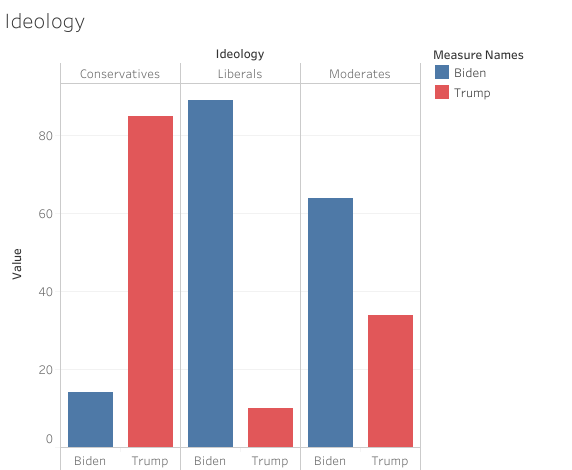
\includegraphics[width=0.6\textwidth]{figures/Ideology.png}
        \caption{Tỷ lệ ủng hộ ứng cử viên theo quan điểm chính trị}
    \end{figure}

    \begin{figure}[h!]
        \centering
        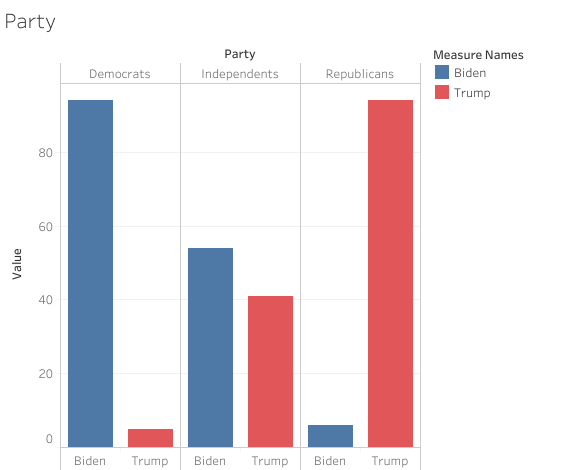
\includegraphics[width=0.6\textwidth]{figures/Party.png}
        \caption{Tỷ lệ ủng hộ ứng cử viên theo đảng phái chính trị}
    \end{figure}

    \begin{figure}[h!]
        \centering
        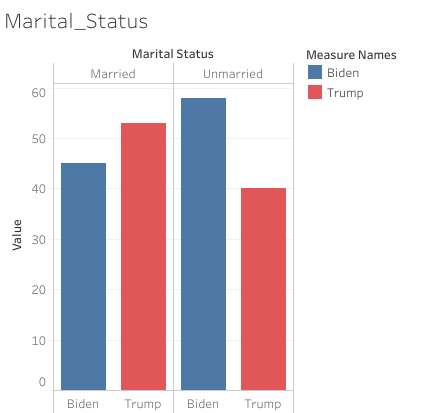
\includegraphics[width=0.6\textwidth]{figures/Marital_Status.png}
        \caption{Tỷ lệ ủng hộ ứng cử viên theo tình trạng hôn nhân}
    \end{figure}

    \begin{figure}[h!]
        \centering
        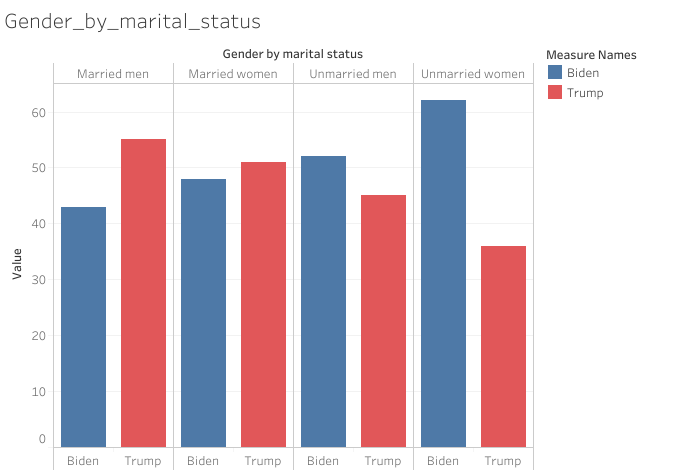
\includegraphics[width=0.6\textwidth]{figures/Gender_by_marital_status.png}
        \caption{Tỷ lệ ủng hộ ứng cử viên theo giới tính và tình trạng hôn nhân}
    \end{figure}

    \begin{figure}[h!]
        \centering
        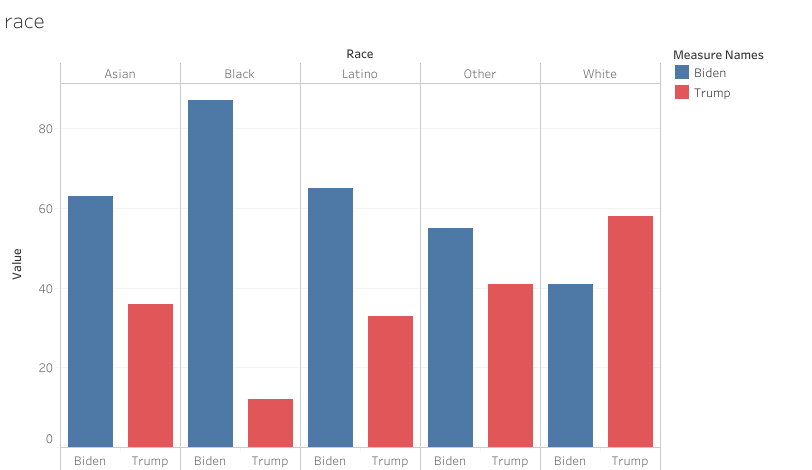
\includegraphics[width=0.6\textwidth]{figures/race.png}
        \caption{Tỷ lệ ủng hộ ứng cử viên theo chủng tộc}
    \end{figure}

    \begin{figure}[h!]
        \centering
        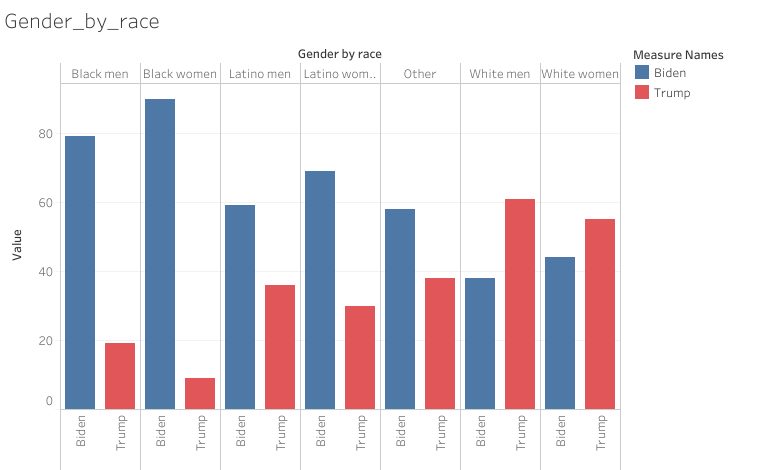
\includegraphics[width=0.6\textwidth]{figures/Gender_by_race.png}
        \caption{Tỷ lệ ủng hộ ứng cử viên theo giới tính và chủng tộc}
    \end{figure}

    \begin{figure}[h!]
        \centering
        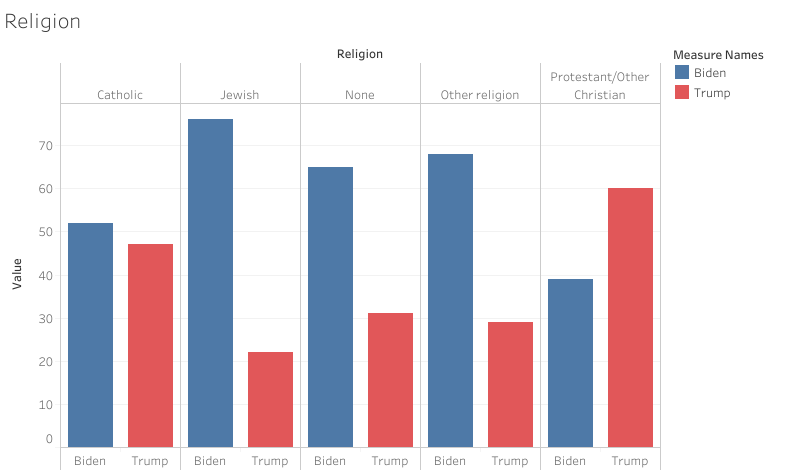
\includegraphics[width=0.6\textwidth]{figures/Religion.png}
        \caption{Tỷ lệ ủng hộ ứng cử viên theo tôn giáo}
    \end{figure}

    \begin{figure}[h!]
        \centering
        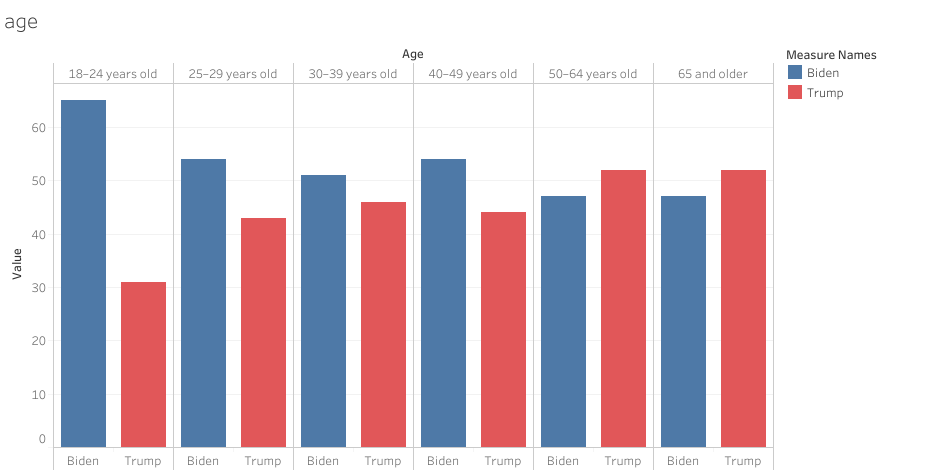
\includegraphics[width=0.6\textwidth]{figures/age.png}
        \caption{Tỷ lệ ủng hộ ứng cử viên theo độ tuổi}
    \end{figure}

    \begin{figure}[h!]
        \centering
        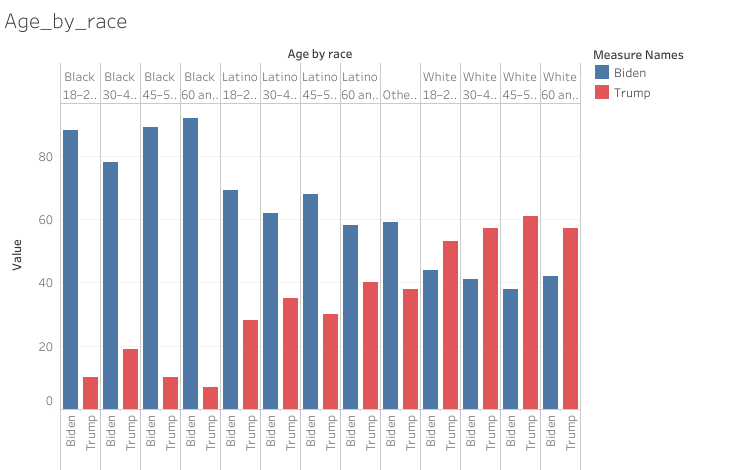
\includegraphics[width=0.6\textwidth]{figures/Age_by_race.png}
        \caption{Tỷ lệ ủng hộ ứng cử viên theo độ tuổi và chủng tộc}
    \end{figure}

    \begin{figure}[h!]
        \centering
        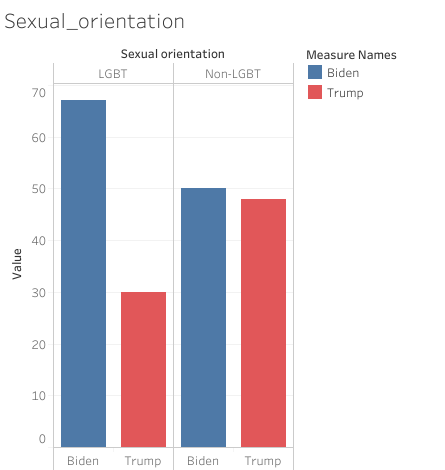
\includegraphics[width=0.6\textwidth]{figures/Sexual_orientation.png}
        \caption{Tỷ lệ ủng hộ ứng cử viên theo xu hướng giới tính}
    \end{figure}

    \begin{figure}[h!]
        \centering
        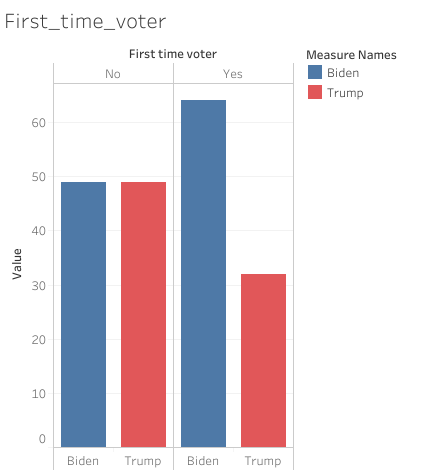
\includegraphics[width=0.6\textwidth]{figures/First_time_voter.png}
        \caption{Tỷ lệ ủng hộ ứng cử viên theo số lần đi bỏ phiếu}
    \end{figure}

    \begin{figure}[h!]
        \centering
        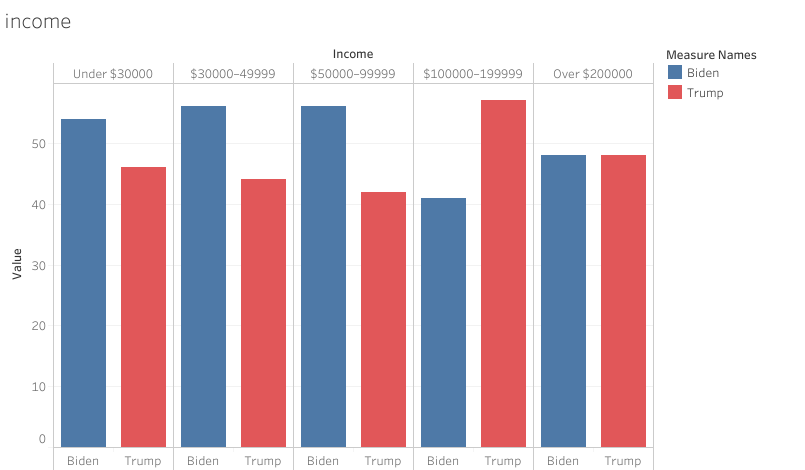
\includegraphics[width=0.6\textwidth]{figures/income.png}
        \caption{Tỷ lệ ủng hộ ứng cử viên theo thu nhập}
    \end{figure}

    \begin{figure}[h!]
        \centering
        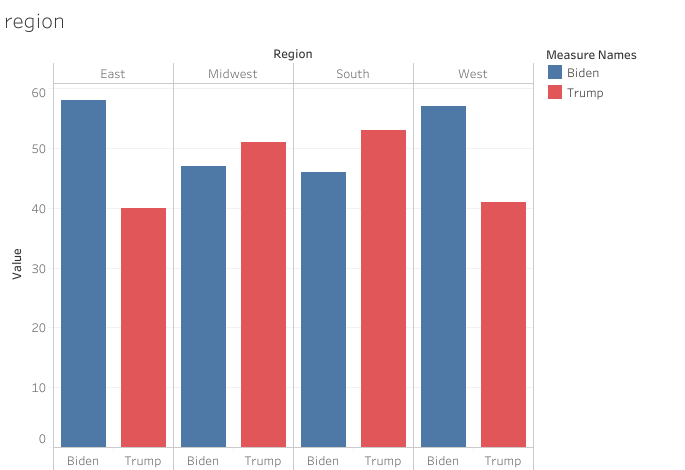
\includegraphics[width=0.6\textwidth]{figures/region.png}
        \caption{Tỷ lệ ủng hộ ứng cử viên theo khu vực}
    \end{figure}

    \begin{figure}[h!]
        \centering
        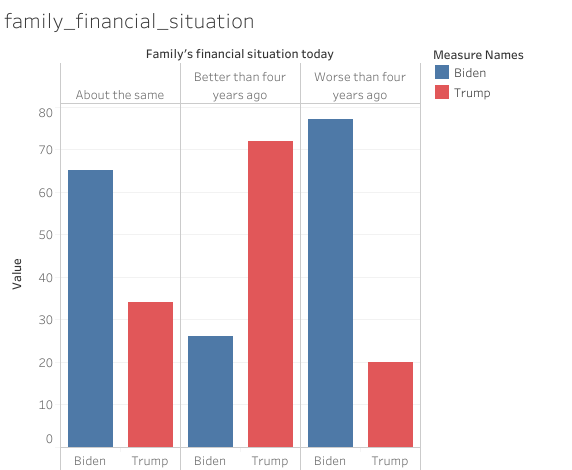
\includegraphics[width=0.6\textwidth]{figures/family_financial_situation.png}
        \caption{Tỷ lệ ủng hộ ứng cử viên theo tình trạng tài chính}
    \end{figure}

    \begin{figure}[h!]
        \centering
        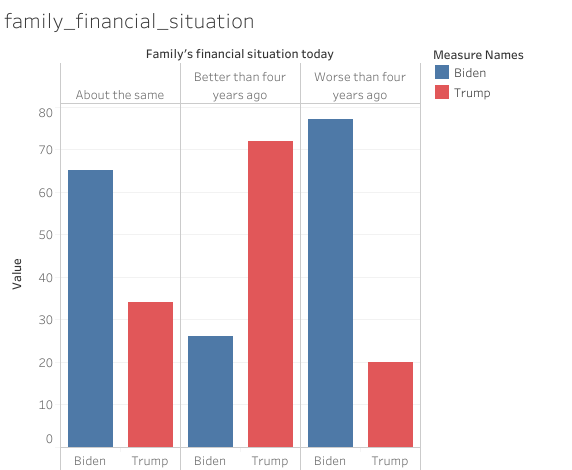
\includegraphics[width=0.6\textwidth]{figures/family_financial_situation.png}
        \caption{Tỷ lệ ủng hộ ứng cử viên theo phục vụ quân ngũ}
    \end{figure}

    \begin{figure}[h!]
        \centering
        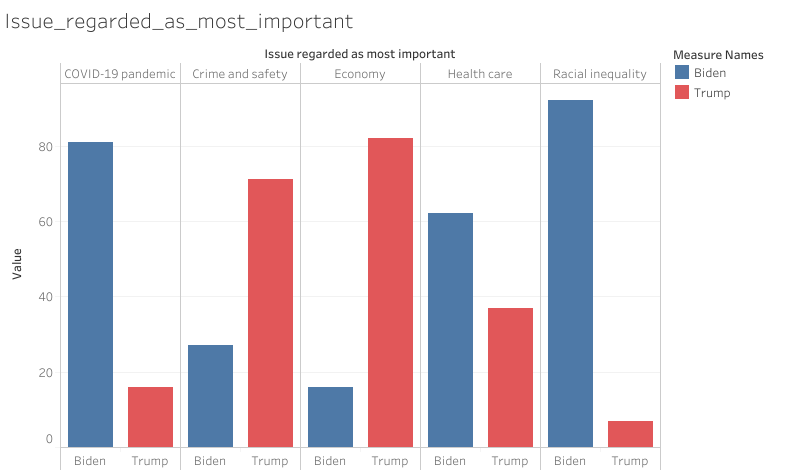
\includegraphics[width=0.6\textwidth]{figures/Issue_regarded_as_most_important.png}
        \caption{Tỷ lệ ủng hộ ứng cử viên theo cách nhìn nhận các vấn đề xã hội}
    \end{figure}

    \begin{figure}[h!]
        \centering
        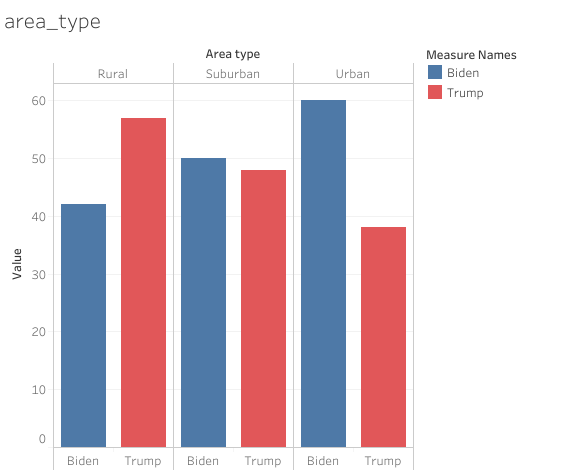
\includegraphics[width=0.6\textwidth]{figures/area_type.png}
        \caption{Tỷ lệ ủng hộ ứng cử viên theo khu vực sinh sống}
    \end{figure}


    \begin{figure}[h!]
        \centering
        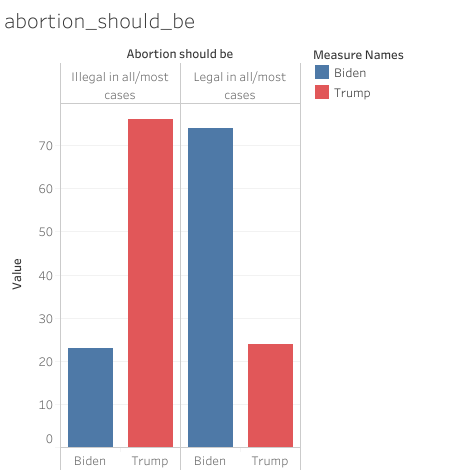
\includegraphics[width=0.6\textwidth]{figures/abortion_should_be.png}
        \caption{Tỷ lệ ủng hộ ứng cử viên theo quan điểm về nạo phá thai}
    \end{figure}

    \begin{figure}[h!]
        \centering
        \begin{subfigure}[b]{\textwidth}
            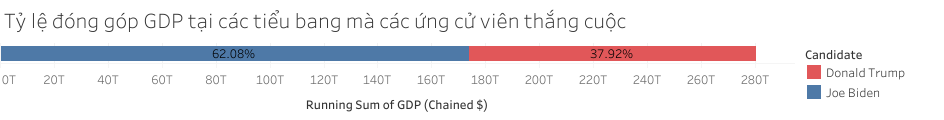
\includegraphics[width=0.9\textwidth]{State_Percentage_GDP_Candidate.png}
            \caption{Tỷ lệ đóng góp GDP tại các tiểu bang mà các ứng cử viên thắng}
        \end{subfigure}
        \vfill
        \begin{subfigure}[b]{\linewidth}
            \includegraphics[width=0.9\linewidth]{State_Percentage_Population_Candidate.png}
            \caption{Tỷ lệ đóng góp dân số tại các tiểu bang mà các ứng cử viên thắng}
        \end{subfigure}
        \vfill
        \begin{subfigure}[b]{\textwidth}
            \includegraphics[width=0.9\linewidth]{County_Total_Percentage_Candidate_Win.png}
            \caption{Tỷ lệ thắng trên các hạt của từng ứng cử viên}
        \end{subfigure}
        \vfill
        \begin{subfigure}[b]{\textwidth}
            \includegraphics[width=0.9\linewidth]{County_Percentage_Population_Candidate.png}
            \caption{Tỷ lệ đóng góp dân số tại các hạt mà các ứng cử viên thắng}
        \end{subfigure}
        \caption{So sánh quy mô dân số và kinh tế tại các bang, hạt các ứng cử viên chiến thắng}
    \end{figure}

\end{document}